\documentclass{article}

%%%%%%%%%%%%%%% LIBRERIAS %%%%%%%%%%%%%%%%%%%%%
\usepackage[thinc]{esdiff}
\usepackage{amsmath}
\usepackage{caption}
\usepackage{physics}
\usepackage{titlesec}
\usepackage{titletoc}
\usepackage{graphicx}
\usepackage[spanish,es-tabla]{babel} % 'es-tabla' cambia Cuadro→Tabla
\usepackage{hyperref}                % cargar después de babel
\usepackage{float}
\usepackage{circuitikz}
\usepackage[left=1.6cm,right=1.6cm,top=1.8cm,bottom=1.8cm]{geometry}
\usepackage{subfiles} 
\usepackage{subcaption}
\usepackage{pgfplots}
\pgfplotsset{compat=1.18}
\usepackage{booktabs} % Para tablas con tematica de paper cientifico
\usepackage{siunitx}  % Para alinear números en las tablas d:

%%%%%%%%%%%%%%%%%%% VARIABLES %%%%%%%%%%%%%%%%%%%%
\newcommand{\Facultad}{Instituto Tecnológico \\de\\ Buenos Aires} %constantes
\newcommand{\TPn}{Trabajo Práctico Final}
\newcommand{\TPtema}{Diseño de PCBs - Simulación}
\renewcommand{\thesection}{\arabic{section}}          % 2
\renewcommand{\thesubsection}{\quad \alph{subsection}}   % a
\renewcommand{\thesubsubsection}{\quad \thesubsection.~\roman{subsubsection}} % a. i
\graphicspath{{imagenes/}} %para que acceda a las fotos en la carpeta directamente


%%%%%%%%%%%%%%%%%% FORMATO TÍTULO Y NUMERACIÓN %%%%%%%%%%%%%%%%%%%
% Numeración de secciones
\renewcommand{\thesection}{\arabic{section}.}          
\renewcommand{\thesubsection}{\thesection\arabic{subsection}}       
\renewcommand{\thesubsubsection}{$\alph{subsubsection}$}

% Numerar hasta subsubsecciones
\setcounter{secnumdepth}{3}

% Formato de títulos
\titleformat{\section}{\LARGE\bfseries}{\thesection}{1em}{}
\titleformat{\subsection}{\large\bfseries}{\thesubsection}{0.5em}{}
\titleformat{\subsubsection}{\large\bfseries}{\thesubsubsection}{0.5em}{}



%%%%%%%%%%%%%%%%%%% ARCHIVO %%%%%%%%%%%%%%%%%%%%%%%%
\begin{document}

%%%CARATULA%%%
\begin{titlepage} %creo portada

        \begin{flushleft}
            \centering
            
\includegraphics[width=0.3\textwidth]{Logo_ITBA.png}
        \end{flushleft}

        \centering
            
        {\scshape\LARGE \Facultad \par} %\par sirve para indicar un final de parrafo
        \vspace{1cm}                    %esto hace un espacio entre lineas de 1cm


        {\huge\bfseries \TPn \par}
        \vspace{1.5cm}
        {\Large Laboratorio de Electrónica\\ 25.13 \par}
        \vspace{0.5cm}
        {\Large \TPtema \par}
        \vfill                      %sirve para rellenar el espacio y quede simétrico.
        {\Large \bfseries Rita Moschini 67026 \par}
        \vspace{12cm}
        

\end{titlepage}

\section{Introducción}
En este documento se muestra el diseño y la simulación de una fuente de alimentación variable regulada mediante un potenciómetro, la cual se alimenta externamente con un transformador de 15VAC, a su vez conectado a la red eléctrica mediante un conector de tipo \texttt{CONIN VAC}.


\section{Simulación}
    \begin{figure}[H]
        \centering
        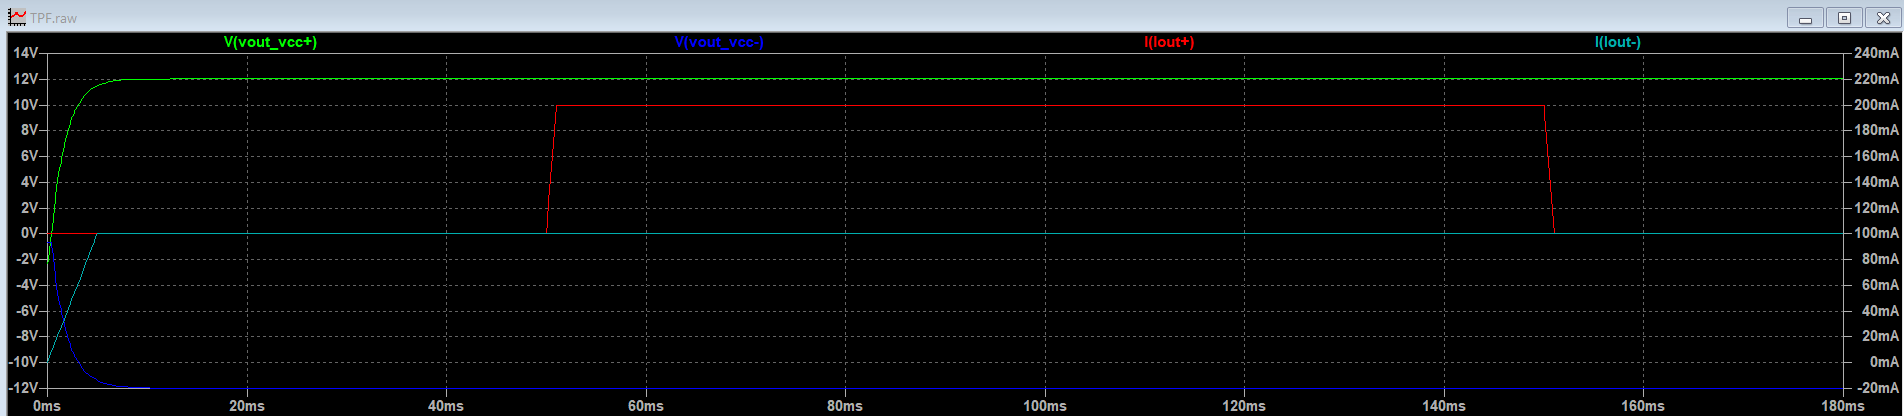
\includegraphics[width=1\textwidth]{imagenes/Escalon_Vout+.png}
        \caption{Variación de tensión en la salida, teniendo una corriente de salida tipo escalón en la
fuente positiva y con 100mA en la negativa}
        \label{fig:simulacionVout+}
    \end{figure}

    \begin{figure}[H]
        \centering
        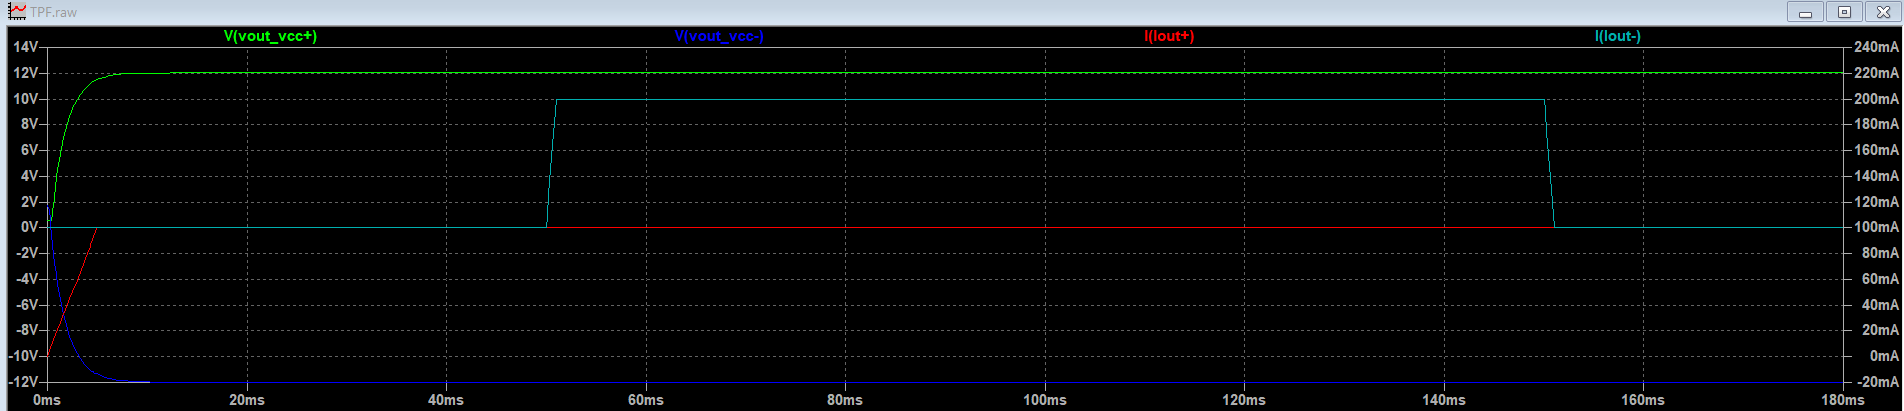
\includegraphics[width=1\textwidth]{imagenes/Escalon_Vout-.png}
        \caption{Variación de tensión en la salida, teniendo una corriente de salida tipo escalón en la
fuente negativa y con 100mA en la positiva}
        \label{fig:simulacionVout-}
    \end{figure}

    \begin{figure}[H]
        \centering
        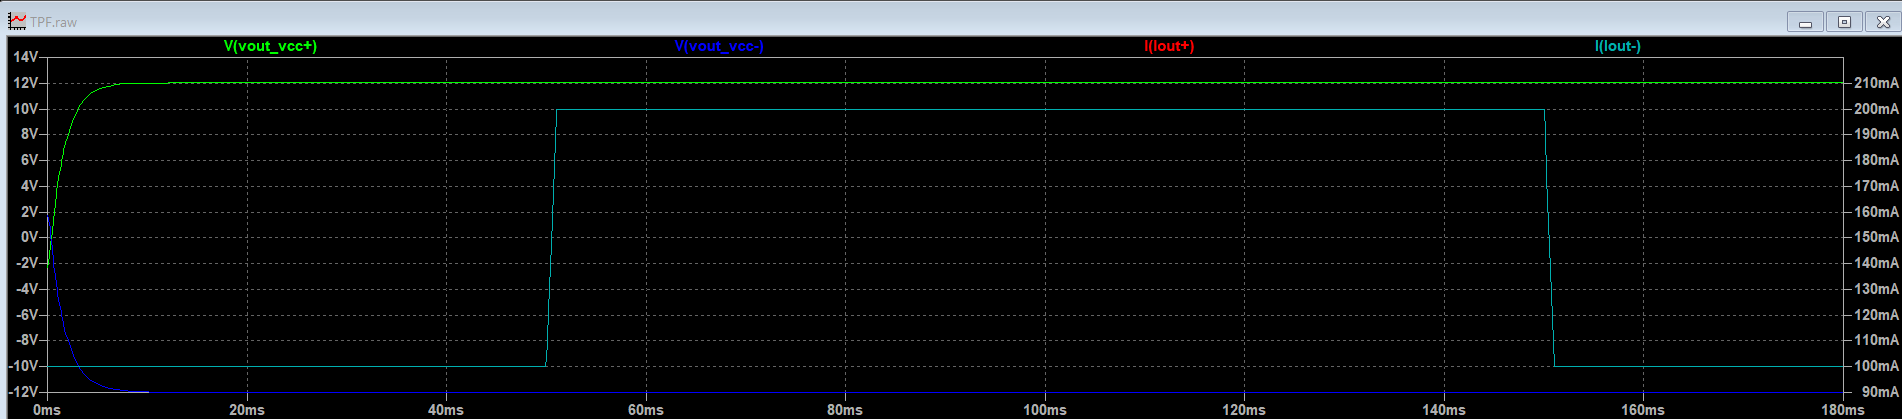
\includegraphics[width=1\textwidth]{imagenes/escalones.png}
        \caption{Variación de tensión en la salida, teniendo una corriente de salida tipo escalón tanto en la
fuente negativa y como en la positiva}
        \label{fig:simulacionVout-_Vout}
    \end{figure}


\section{Desarrollo del PCB}

\subsection{Esquemático}
    \begin{figure}[H]
        \centering
        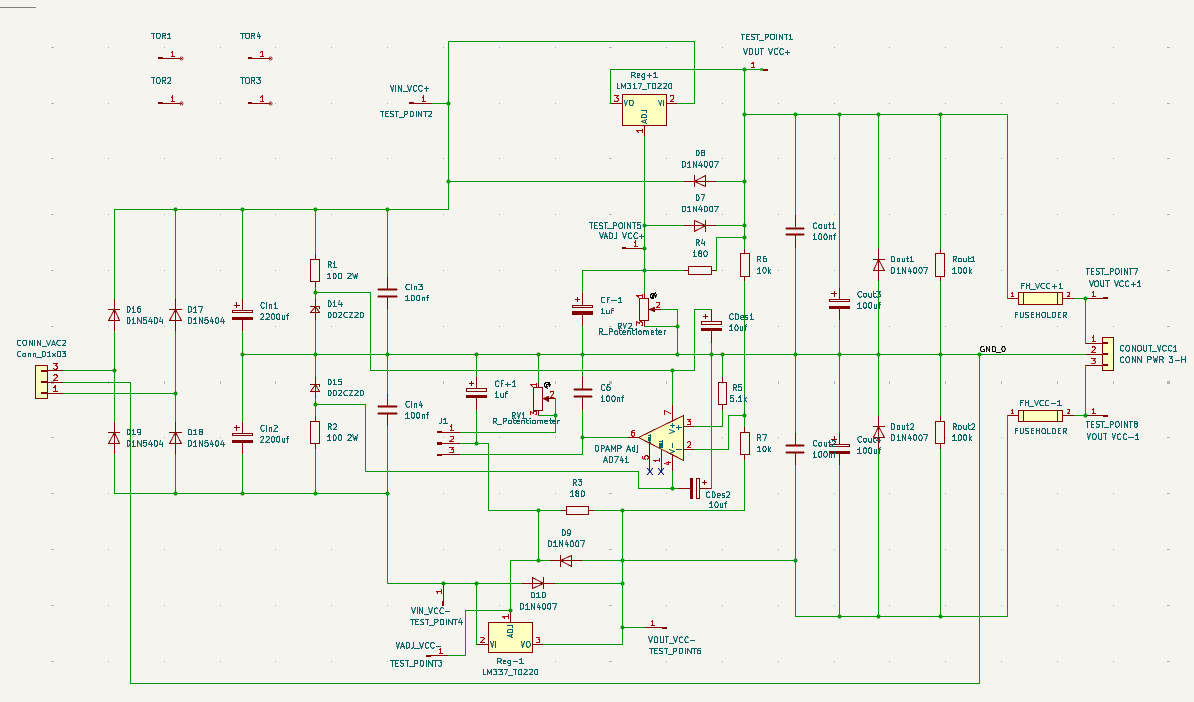
\includegraphics[width=1\textwidth]{imagenes/esquematico.png}
        \caption{Esquemático}
        \label{fig:esquematico}
    \end{figure}

\subsection{Diseño del Layout}
    \begin{figure}[H]
        \centering
        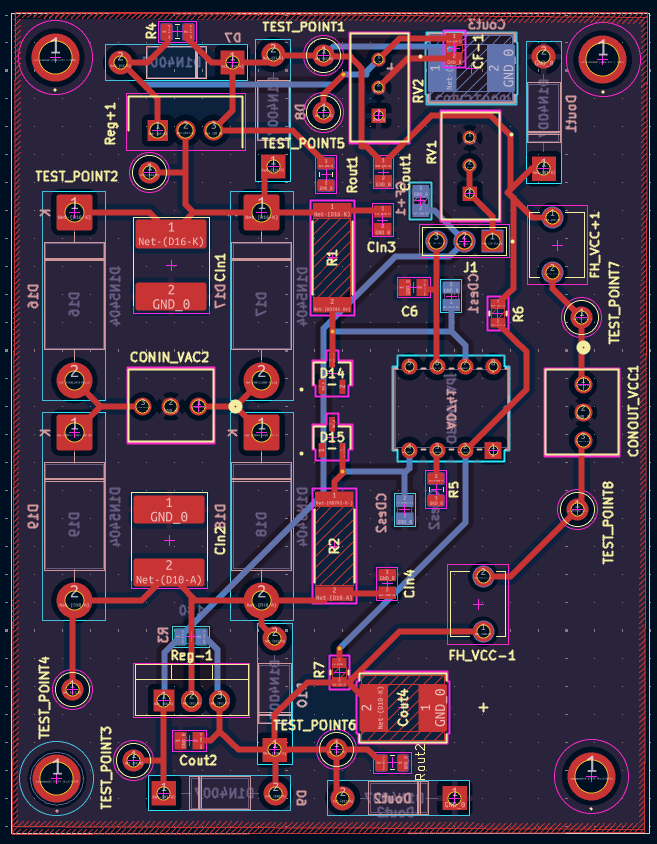
\includegraphics[width=0.6\textwidth]{imagenes/pcb_completo.png}
        \caption{PCB con todas las capas visibles.}
        \label{fig:pcb_completo}
    \end{figure}


    \begin{figure}[H]
        \centering
        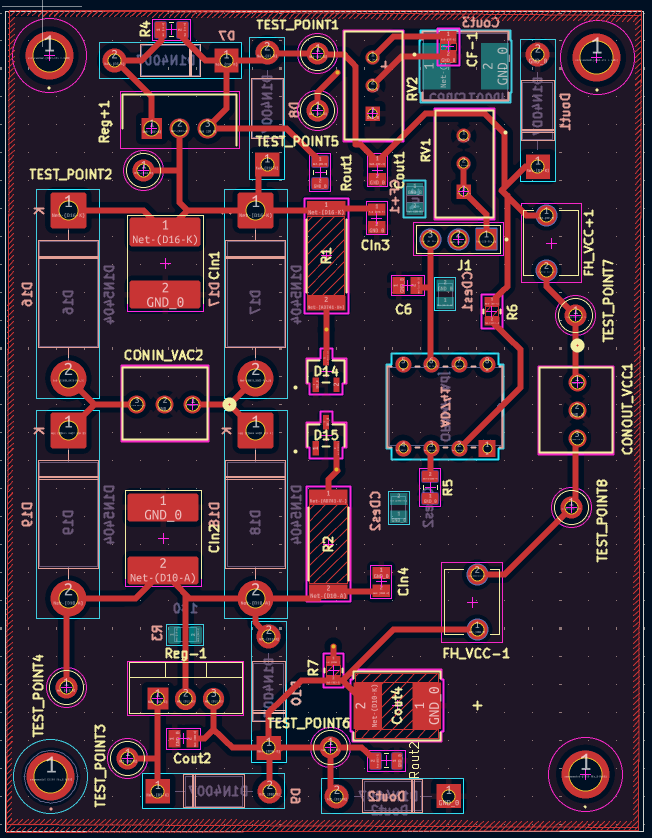
\includegraphics[width=0.6\textwidth]{imagenes/pcb_frontLayer.png}
        \caption{PCB con todas las capas visibles excepto la Bottom Layer.}
        \label{fig:pcb_frontLayer}
    \end{figure}


    \begin{figure}[H]
        \centering
        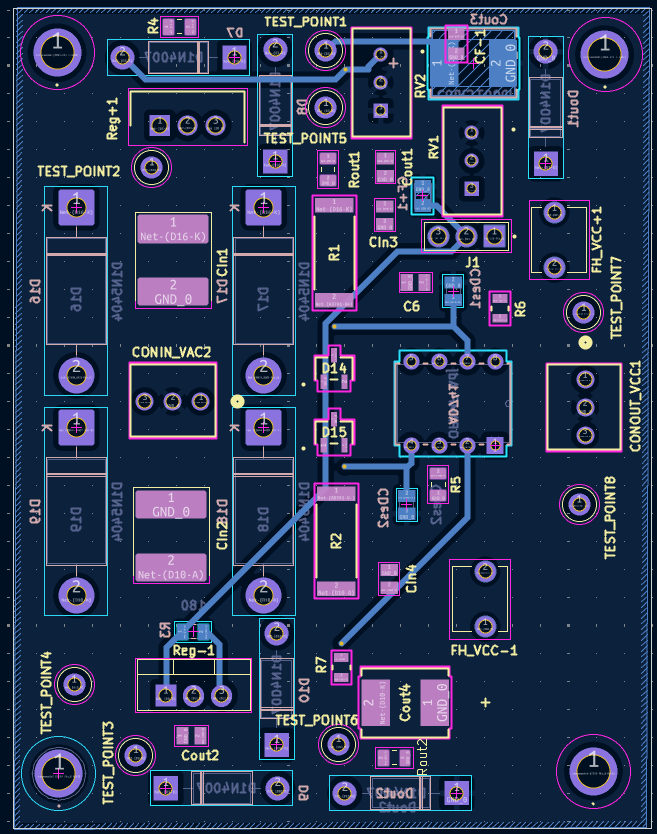
\includegraphics[width=0.6\textwidth]{imagenes/pcb_bottomLayer.png}
        \caption{PCB con todas las capas visibles excepto la Front Layer.}
        \label{fig:pcb_bottomLayer}
    \end{figure}






\end{document}